\documentclass{article}

\usepackage[utf8]{inputenc}
\usepackage{amssymb}
\usepackage{amsmath}
\usepackage{mathabx}
\usepackage{dcolumn}
\usepackage{geometry}
\usepackage{breqn}
\usepackage{graphicx}
\usepackage{float}
\usepackage{mathrsfs}
\usepackage{array}
\usepackage{caption}
\usepackage{subcaption}
\usepackage[spanish,es-lcroman]{babel}
\decimalpoint
\usepackage{enumerate}
\usepackage{nicefrac} 
\usepackage[most]{tcolorbox}
\usepackage{tcolorbox} % For solution boxes
%\decimalpoint
\setlength\parindent{0pt}
\usepackage{enumitem}
\newcommand*{\QED}{\hfill\ensuremath{\blacksquare}}
\usepackage{authblk}
\selectlanguage{spanish}
\geometry{letterpaper, margin=1in}
\pagestyle{headings}
\usepackage{amsthm} 
\newtheorem{theorem}{Teorema}[section]
\newtheorem{corollary}{Corolario}[theorem]
\newtheorem{lemma}[theorem]{Lema}
\theoremstyle{remark}
\newtheorem*{remark}{Considere}
\DeclareUnicodeCharacter{2212}{-}
\usepackage{epigraph}

\usepackage[backend=biber, style=apa]{biblatex}
\addbibresource{bib/ref_entrega2.bib}

\usepackage{tikz}
\usepackage{hyperref}

\tcbset{colback=blue!10, 
    %colframe=green!45!black!20, 
    colframe=blue!70!black!70, 
    title=Soluci\'on,
    fonttitle=\bfseries,  
    coltitle=white,
    standard jigsaw, opacityback=50, arc=0mm, breakable} 

\newcommand{\ubar}[1]{\text{\b{$#1$}}}
 
\theoremstyle{definition}
\newtheorem{definition}{Definici\'on}[section]

\title{\textbf{Macroeconom\'ia Avanzada de Largo Plazo} \\ \textbf{Taller 2 - Parte Grupal}}

\author{Jhoan Sebasti\'an Fuentes Hern\'andez \and Nicolas Lozano Huertas}
\date{2025-10}

\begin{document}
\maketitle
\vspace{-1 cm}
\section*{[100 puntos] Parte 2: Trabajo de Investigación}

\noindent El objetivo de esta parte es transformar sus intuiciones y hallazgos empíricos del Taller 1 en un modelo formal que les permita analizar dinámicas, realizar análisis comparativos, calibrar y explorar contrafactuales.

\begin{enumerate}
    \item ¿Cuáles son los principales conflictos o tensiones (``\emph{trade offs}'') que identificaron en el Taller 1 para su tema de interés? \\
        \begin{tcolorbox}[title= Solución Punto 1 (Revisado - Versión Preferida)]

El análisis del impacto económico de la Inteligencia Artificial (IA) requiere identificar las tensiones fundamentales que enfrentan los agentes económicos o que emergen a nivel agregado. Para nuestro tema de interés, identificamos los siguientes \textit{trade-offs} clave:

\begin{enumerate}
    \item \textbf{Eficiencia Productiva vs. Desplazamiento Laboral (TR/TA):}
        \begin{itemize}
            \item \textbf{Agente Decisor Primario:} Empresas (modeladas como minimizadoras de costos o maximizadoras de beneficios).
            \item \textbf{Decisión Microeconómica:} ¿Invertir y adoptar tecnología IA para automatizar Tareas Rutinarias (TR) y/o Tareas Analíticas (TA), si esto reduce el costo unitario de producción por debajo del costo laboral ($w_M, w_A$)?
            \item \textbf{Trade-off a Nivel de Empresa:} El beneficio directo es una mayor eficiencia y reducción de costos (potencialmente reflejado en mayores márgenes, mayor producción o menores precios, con ahorros $\pi_M, \pi_A$). La "contrapartida" no es un costo directo para la empresa optimizadora, sino una \textit{consecuencia agregada} en el mercado laboral.
            \item \textbf{Consecuencia Agregada (Equilibrio de Mercado):} La adopción generalizada de IA para TR/TA por parte de las empresas reduce la demanda agregada por trabajadores Manuales/Rutinarios (M) y Analíticos (A), ejerciendo presión a la baja sobre sus salarios relativos ($w_M, w_A$) y alterando la distribución funcional del ingreso (hacia el capital/IA).
        \end{itemize}
        \vspace{0.5em} % Espacio entre elementos principales

    \item \textbf{Optimización de Costos (IA) vs. Valor de la Interacción Humana (TS):}
        \begin{itemize}
            \item \textbf{Agente Decisor Primario:} Empresas (al diseñar procesos y elegir insumos para Tareas Socioemocionales/Interacción - TS).
            \item \textbf{Influencia Secundaria:} Preferencias de los Consumidores (que pueden valorar la interacción humana).
            \item \textbf{Decisión Microeconómica (Empresa):} Para tareas TS, ¿utilizar IA (si es técnicamente viable y potencialmente más barata/escalable) o emplear trabajadores Socioemocionales (S) (potencialmente más costosos pero que aportan un valor diferencial)?
            \item \textbf{Trade-off a Nivel de Empresa:} Minimizar costos operativos (favorece IA si es capaz y barata) vs. Preservar/Aumentar el valor del servicio satisfaciendo una demanda explícita o implícita por interacción humana (favorece a S). Esto último puede permitir precios más altos, mayor lealtad del cliente, o ser intrínseco a la calidad del servicio. El modelo deberá capturar esto vía supuestos sobre la productividad relativa ($\psi_S \gg \psi_k$ en TS) y/o incorporando preferencias del consumidor que afecten la demanda del bien final si este requiere tareas TS.
        \end{itemize}
        \vspace{0.5em}

    \item \textbf{Reasignación de Tareas Inducida por IA y Escasez Relativa de Habilidades:}
        \begin{itemize}
            \item \textbf{Fenómeno:} Este no es un \textit{trade-off} de decisión directa para un agente único, sino un \textbf{resultado clave del equilibrio general} tras la adopción de IA.
            \item \textbf{Mecanismo:} Las decisiones de las empresas de automatizar TR y TA (basadas en el trade-off \#1) reducen la demanda de trabajo M y A. Si la tecnología IA tiene límites en su capacidad para realizar tareas TS y TJ (Tareas de Juicio), y estas tareas siguen siendo esenciales en la producción (determinadas por la estructura productiva, ej. parámetro $\lambda$), la demanda por trabajadores S y J persiste.
            \item \textbf{Resultado Agregado:} La \textbf{escasez relativa} de las habilidades S y J frente a una demanda sostenida (mientras M y A se vuelven relativamente abundantes por el desplazamiento) tiende a elevar los salarios relativos $w_S$ y $w_J$ en comparación con $w_M$ y $w_A$. El modelo captura esta dinámica a través de la interacción entre la asignación de tareas (endógena o exógena en la versión simplificada) y el mecanismo de vaciado del mercado laboral que determina los salarios.
        \end{itemize}
        \vspace{0.5em}

    \item \textbf{Alcance de la Automatización vs. Responsabilidad y Juicio Humano (TJ):}
         \begin{itemize}
            \item \textbf{Agente Decisor:} Empresas (primariamente) y/o Sociedad/Regulador (imponiendo límites).
            \item \textbf{Decisión Microeconómica (Empresa):} ¿Delegar Tareas de Juicio (TJ) –críticas, con implicaciones éticas o de alta responsabilidad– a una IA, incluso si fuera técnicamente posible y eficiente en costos?
            \item \textbf{Trade-off a Nivel de Empresa:} Maximización de eficiencia/beneficios vs. Mitigación de riesgos (legales, reputacionales, éticos, fallos catastróficos) asociados a la falta de juicio, responsabilidad o transparencia de la IA en tareas críticas.
            \item \textbf{Restricción Social/Institucional:} La sociedad puede imponer límites explícitos a la automatización de ciertas TJ (ej. $TJ \cap T_k = \emptyset$), reflejando una preferencia colectiva por mantener el control y la rendición de cuentas humanas. Esto se modela como una \textbf{restricción exógena} sobre la asignación de tareas.
            \item \textbf{Trade-off Social:} Potencial de productividad económica máxima vs. Mantenimiento de salvaguardas éticas, de seguridad y responsabilidad.
        \end{itemize}
\end{enumerate}

\vspace{1em} % Espacio antes de la conclusión

La identificación precisa de estos \textit{trade-offs} es clave para guiar la estructura del modelo formal. Los \textit{trade-offs} \#1 (Eficiencia/Desplazamiento) y \#4 (Automatización/Juicio) informan directamente las reglas de optimización y las restricciones que enfrentan las empresas al asignar tareas. El \textit{trade-off} \#2 (Costo/Valor Humano) subraya la importancia de modelar adecuadamente las capacidades relativas de IA y humanos en tareas socioemocionales, potencialmente incorporando preferencias del consumidor o simplemente reflejándolo en las funciones de productividad ($\psi$). Finalmente, el fenómeno \#3 (Reasignación/Escasez Relativa) no es una elección directa, sino un resultado central del equilibrio de mercado que el modelo debe ser capaz de generar (o analizar, en su versión simplificada) para evaluar las consecuencias distributivas de la IA. Estos elementos definen los mecanismos económicos que el modelo formal buscará capturar.

\end{tcolorbox}
    
    \item ¿Cómo se relacionan los \emph{trade-offs} identificados en el Taller 1 con los supuestos de comportamiento de los agentes en un modelo teórico? Explique qué aspectos (por ejemplo, preferencias, restricciones tecnológicas o institucionales) son claves para capturar estas dinámicas.

        \begin{tcolorbox}[title= Soluci\'on 2]
            \begin{enumerate}

                \item \textbf{Contexto: } 

                \begin{description}[labelsep=1em]
                  \item[Empresas (Productores):] Buscan minimizar costos (dados la tecnolog\'\i a y los precios de los factores) para producir las tareas y  el bien final $y$. Toman decisiones sobre qu\'e tecnolog\'\i a usar y qu\'e factor asignar a cada tarea.
                  \item[Trabajadores/Hogares (Tipos $A$, $S$, $J$, $M$):] Ofrecen su trabajo (asumimos que es inel\'astico $\ell_g$ para $g\in\{A,S,J,M\}$) y consumen el producto neto $c$. Se especializan en distintas categor\'\i as de tareas (\emph{A} en $T_A$, \emph{S} en $T_S$, \emph{J} en $T_J$, \emph{M} en $T_R$). Su oferta es pasiva.
                  \item[Sociedad/Regulador (Potencial):] Imponen reglas o restricciones externas a la automatizaci\'on.
                \end{description}
            \item \textbf{Eficiencia/Productividad vs. Desplazamiento/Desigualdad}
              \begin{itemize}
                \item \emph{Agente y comportamiento}: Decisi\'on de las Empresas de minimizar costos. Cuando la automatizaci\'on reduce el costo efectivo $C_k(x)$ de realizar una tarea $x$ (sea $T_R$ o $T_A$) por debajo del costo de realizarla con el trabajo correspondiente ($C_M(x)$ para $T_R$, $C_A(x)$ para $T_A$), la empresa reasigna la tarea al capital.
                \item \emph{Aspectos cruciales}:
                  \begin{itemize}
                    \item \textbf{Restricciones tecnol\'ogicas}: Existencia y mejora del capital con capacidad de automatizaci\'on ($\psi_k(x)$, $q(x)$) que la hace posible y rentable. La magnitud del ahorro de costos ($\pi_M$, $\pi_A$) es tambi\'en tecnol\'ogica.
                    \item \textbf{Supuestos de comportamiento (Empresas)}: Se asume que las empresas optimizan y adoptan m\'etodos que reducen costos.
                    \item \textbf{Estructura de producci\'on}: La reasignaci\'on de tareas afecta la demanda laboral agregada $\Gamma_g$ y la productividad total $y$, seg\'un la funci\'on CES y el par\'ametro $\lambda$.
                  \end{itemize}
              \end{itemize}
            
              \item \textbf{Costo/Eficiencia de automatizr vs. Valor de la Interacci\'on Humana (Trabajador $S$)}
              \begin{itemize}
                \item \emph{Agente y comportamiento}: Decisi\'on de las Empresas sobre c\'omo producir tareas de interacci\'on $T_S$, potencialmente influida por las preferencias de los consumidores.
                \item \emph{Aspectos cruciales}:
                  \begin{itemize}
                    \item \textbf{Restricciones tecnol\'ogicas}: Se supone que hay l\'imites para la automatizaci\'on de $T_S$ ($\psi_k(x)$ bajo/cero para $x\in T_S$), mientras que los trabajadores $S$ presentan alta productividad ($\psi_S(x)$ alto). Los tipos $M$, $A$ y $J$ se asumen de baja productividad en $T_S$.
                    \item \textbf{Estructura de producci\'on}: Necesidad de las tareas $T_S$ para producir $y$ (depende de $\lambda$).
                    \item \textbf{Preferencias}: Una prima del consumidor por servicio ``humanizado'' afectar\'\i a la demanda y la decisi\'on de la empresa m\'as all\'a de solo el costo.
                    \item \textbf{Supuestos de comportamiento (Empresas)}: \textquestiondown Responden solo a costos o tambi\'en a la disposici\'on a pagar?
                  \end{itemize}
              \end{itemize}
            
              \item \textbf{Retorno a la Automatizaci\'on ($T_R/T_A$) vs. Retorno a Habilidades Humanas ($T_S/T_J$)}
              \begin{itemize}
                \item \emph{Agente y comportamiento}: Resultado agregado de las decisiones de asignaci\'on de todas las Empresas, que determina los salarios de mercado $w_A, w_S, w_J, w_M$.
                \item \emph{Aspectos cruciales}:
                  \begin{itemize}
                    \item \textbf{Restricciones tecnol\'ogicas (diferenciales)}: La automatizaci\'on impacta diferencialmente las categor\'\i as de tareas (mucho a $T_R/T_A$, poco o nada a $T_S/T_J$).
                    \item \textbf{Ventaja comparativa}: Especializaci\'on de los trabajadores en distintas tareas ($\psi_g(x)$), lo que vincula el impacto tecnol\'ogico sobre tareas a grupos espec\'\i ficos.
                    \item \textbf{Sustituibilidad $\lambda$}: Grado de complementariedad entre tareas. Si $T_S/T_J$ son poco sustituibles por $T_R/T_A$, su valor relativo aumentar\'\i a cuando \'estas \'ultimas se automaticen.
                    \item \textbf{Supuestos de comportamiento}: El mercado laboral ajusta los salarios para igualar oferta fija $\ell_g$ y demanda derivada de $\Gamma_g$.
                  \end{itemize}
              \end{itemize}
            
              \item \textbf{Alcance de la Automatizaci\'on vs. Responsabilidad/Juicio Humano (Trabajador $J$)}
              \begin{itemize}
                \item \emph{Agente y comportamiento}: Decisi\'on de no automatizar tareas cr\'\i ticas ($T_J$) por parte de las Empresas o restricci\'on institucional impuesta por la Sociedad.
                \item \emph{Aspectos cruciales}:
                  \begin{itemize}
                    \item \textbf{Restricciones tecnol\'ogicas}: Se supone $\psi_k(x)=0$ (o costo infinito) para $x\in T_J$; solo los trabajadores $J$ pueden realizarlas ($\psi_J(x)$ alto).
                    \item \textbf{Restricciones institucionales}: Regla expl\'\i cita $T_J\cap T_k=\varnothing$.
                    \item \textbf{Supuestos de comportamiento}: Una versi\'on avanzada podr\'\i a incluir aversi\'on al riesgo que justifique no automatizar $T_J$ incluso si fuera t\'ecnicamente posible.
                  \end{itemize}
              \end{itemize}
            \end{enumerate}
            
            \textbf{Conclusi\'on} \\
            Para capturar estas din\'amicas en el modelo enriquecido (con trabajadores $M$), los aspectos cruciales son:
            \begin{itemize}
              \item \textbf{Restricciones tecnol\'ogicas}: Definir capacidades y l\'imites para la automatizaci\'on ($\psi_k(x), q(x)$) en $T_R, T_A, T_S, T_J$; las habilidades de los cuatro tipos de trabajadores ($\psi_g(x)$) y la estructura de producci\'on (par\'ametro $\lambda$).
              \item \textbf{Supuestos de comportamiento}: Las empresas minimizan costos.
              \item \textbf{Preferencias}: Potencialmente relevantes para el \emph{trade\,-off} \#2.
              \item \textbf{Restricciones institucionales}: Forma directa de modelar l\'imites sociales/\'eticos a la automatizaci\'on (\emph{trade\,-off} \#4).
            \end{itemize}
            
            El modelo permtie que las empresas optimicen sujetas a estas restricciones; el equilibrio de mercado determina los salarios $w_A, w_S, w_J, w_M$ y la asignaci\'on final de tareas $(T_A, T_S, T_J, T_M, T_k)$, revelando c\'omo se resuelven (o no) los \emph{trade\,-offs}, incluido el impacto expl\'\i cito sobre los trabajadores rutinarios/manuales.

        \end{tcolorbox}
    
    \item Desarrolle un modelo formal sencillo que incorpore el mecanismo teórico propuesto en la primera asignación.
        \begin{tcolorbox}[title= Soluci\'on 3]
            Para la construcci\'on de nuestro modelo, decidimos seguir un enfoque de tareas, similar al propuesto por Acemoglu y Restrepo (2022). Este modelo busca mostrar el impacto de la automatizaci\'on en la aignaci\'on de tareas y salarios, considerando diferentes tipos de habilidades laborales.
            \begin{itemize}
                \item \textbf{\textit{Par\'ametros}}
                    \begin{itemize}
                        \item $T$: Conjunto de todas las tareas existentes ($x\in T$). Dividimos este conjunto en: \\
                        $TA$ - tareas intensivas en habilidades anal\'iticas, \\ 
                        $TS$ - tareas intensivas en habilidades socioemocionales, \\
                        $TJ$ - tareas intensivas en habilidades de juicio, \\
                        $TR$ - tareas repetitivas. \\
                        Asumimos que $T=TR \ \cup \ TA \ \cup \ TS \ \cup \ TJ$, donde $TJ \ \cap \  TI = \emptyset \ \ \forall J,I\in \{A,R,S,J\}, J \neq I$.
                        \item $M$: Medida del total de tareas utilizadas en la producci\'on. Normalizamos $M=1$. 
                        \item $G=\{A,S,J,M\}$: Conjunto de los tipos de habilidades (trabajos).
                        \item $l_A$, $l_S$, $l_J$, $l_M$: Oferta total (fija e inel\'astica) de cada tipo de trabajo.
                        \item $\lambda$: Elasticidad de sustituci\'on de los bienes intermedios $y(x)$ en la producci\'on total $y$.
                        \item $A_A$, $A_S$, $A_J$, $A_M$: Par\'ametros de eficiencia/productividad para cada tipo de trabajo.
                        \item $A_k$: Par\'ametros de eficiencia/productividad para el capital.
                        \item $\psi_{g(x)}$: Productividad de cada tipo de trabajo en la realizaci\'on de la tarea $x$. $g \in \{A,S,J,M\}$. 

                        \textbf{Supuesto de especializaci\'on:}

                            \begin{itemize}
                                \item $\psi_{A(x)}$ es alta para $x \in \{TA,TR\}$, y baja para $x \in \{TS,TJ\}$.
                                \item $\psi_{S(x)}$ es alta para $x \in \{TS\}$, y baja para $x \in \{TA,TR,TJ\}$.
                                \item $\psi_{J(x)}$ es alta para $x \in \{TJ\}$, y baja para $x \in \{TA,TS,TR\}$.
                                \item $\psi_{M(x)}$ es alta para $x \in \{TR\}$, y baja para $x \in \{TA,TS,TJ\}$.
                            \end{itemize}
                            
                        \item $\psi_{k(x)}$: Productividad del capital en la realizaci\'on de la tarea $x$. $g \in \{A,S,J\}$.
                            \begin{itemize}
                                \item \textbf{Impacto de la automatizaci\'on:} $\psi_{k(x)}$ es alta o creciente para $x \in \{TR,TA\}$
                                \item \textbf{L\'imites de la automatizaci\'on:} $\psi_{k(x)}$ baja o cero para $x \in \{TS,TJ\}$
                            \end{itemize}
                        \item $q(x)$: Productividad en la producci\'on de capital para la tarea $x$. \emph{Se asume constante e igual a 1}.
                        \item $1/q(x)$: Costo marginal de la producci\'on de capital para la tarea $x$.
                    \end{itemize}
                
                \item {\textbf{\textit{Variables end\'ogenas}}}
                    \begin{itemize}
                        \item $Y$: Producci\'on del bien final (numerario, $P_y=1$).
                        \item $c$: Consumo neto agregado.
                        \item $Y(x)$: Producci\'on intermedia de la tarea $x$.
                        \item $w_A$, $w_S$, $w_J$, $w_M$: Salarios reales de los trabajadores, diferenciados por su habilidad.
                        \item $k(x)$: Cantidad de capital asignado a la tarea $x$.
                        \item $l_{A(x)}, l_{S(x)}, l_{J(x)}, l_{M(x)}$: Cantidad de trabajo de cada tipo asignada a la tarea $x$.
                        \item $T_A$, $T_S$, $T_J$, $T_M$: Conjuntos de tareas asignadas en equilibrio a cada tipo de trabajo.
                        \item $T_k$: Conjunto de tareas asignadas en equilibrio al capital.
                        \item $\Gamma_A$, $\Gamma_S$, $\Gamma_J$, $\Gamma_M$: Proporci\'on del total de tareas realizadas por cada tipo de trabajo.
                        \item $\Gamma_K$: Proporci\'on del total de tareas realizadas por capital.
                        \item $s_K$: Participaci\'on del capital en el producto final.
                    \end{itemize}
                    
                \item {\textbf{\textit{Problema de optimizaci\'on de los agentes.}}} 
                    \begin{itemize}
                        \item \textbf{Empresas (a nivel tarea):} Para cada tarea $x$, las empresas eligen un \'unico factor de producci\'on para realizarla. La empresa elige el factor $i \in \{k,l_A,l_S,l_J\}$ que minimiza el costo unitario de producir $y(x)$, sujeto a la disponibilidad de tecnolo\'ia y otras restricciones. \\
                        Las funciones de costo unitario estan dadas por:
                        \begin{align*}
                            C_{g(x)} &= \frac{w_{g(x)}}{(A_g\psi_{g(x)})} \\
                            C_{k(x)} &= \frac{1/q(x)}{(A_k\psi_{k(x)})}
                        \end{align*}
                        \item \textbf{Empresas (a nivel agregado):} Eligen los niveles de producci\'on de tares ($y(x)$) y la inversi\'on en capital ($k(x)$) para maximizar la producci\'on neta: 
                        $$c=y-\int_T\left(\frac{k(x)}{q(x)}\right)dx$$ 
                        Esto en un contexto de equilibrio competitivo es equivalente a que los factores son remunerados seg\'un su productividad marginal.
                    \end{itemize}
                \item {\textbf{\textit{Caracter\'isticas matemáticas de las funciones que componen los problemas de optimizaci\'on.}}}
                    \begin{itemize}
                        \item \textbf{Funci\'on de producci\'on agregada ($y$):} se utiliza una funci\'on de agregaci\'on tipo CES est\'andar. Esta funci\'on es continua, con rendimientos constantes a escala y cuasic\'oncava.
                            \begin{align*}
                                y=\left[\frac{1}{M}\int_T\left(M\cdot y(x)\right)^{\frac{\lambda-1}{\lambda}}dx\right]^{\frac{\lambda}{\lambda-1}}
                            \end{align*}
                        \item \textbf{Funci\'on de Producci\'on de Tarea (bienes intermedios $y(x)$ utilizados en la producci\'on final):} se utiliza una una funci\'on lineal en los insumos que \emph{pueden} realizarla.
                        \begin{align*}
                            y(x)=A_k*\psi_{k(x)}*k(x) + \sum_{g \in G}\left(A_g\psi_{g(x)}l_{g(x)}\right)
                        \end{align*}
                        \item \textbf{Funci\'on de Costo de producci\'on del Capital:}
                        \begin{align*}
                            costo_k = \frac{1}{q(x)}
                        \end{align*}
                        Donde $q(x)>0$ para las tareas donde el capital es relevante.
                    \end{itemize}
                \item {\textbf{\textit{Restricciones de la econom\'ia.}}}
                    \begin{itemize}
                        \item \textbf{Mercado del bien final:} La producci\'on se consume o se usa para crear capital.
                            \begin{align*}
                                y = c+\int_T\left(\frac{k(x)}{q(x)}\right)dx.
                            \end{align*}
                        \item \textbf{Mercado de Trabajo:} La demanda total de trabajo tipo $g\in G$ debe igualar su oferta fija $l_g$.
                            \begin{align*}
                                \int_{T_g} l_{g(x)} dx = l_g
                            \end{align*}
                        \item \textbf{Mercado de Capital:} El capital $k(x)$ demandado para la tarea $x$ es igual al capital producido para esa tarea.
                        \item \textbf{Restricci\'on de Automatizaci\'on para Tareas de Juicio:} Las tareas intensivas en habilidades de juicio, no pueden ser automatizadas (i.e. asignadas al capital):
                        $$C_{k(x)} > C_{J(x)} \ \forall x \in TJ$$
                        \item \textbf{(Opcional) Restricci\'on de Automatizaci\'on para Tareas Socioemocionales:} Las tareas intensivas en habilidades socioemocionales, no pueden ser automatizadas (i.e. asignadas al capital):
                        $$C_{k(x)} > C_{S(x)} \ \forall x \in TS$$
                    \end{itemize}
            \end{itemize}
        \end{tcolorbox}
    
    \item Derive las condiciones de optimalidad de su modelo (por ejemplo, la ecuación de Euler, condiciones de indiferencia, o las condiciones de equilibrio de mercado) y discuta cómo estas condiciones reflejan los trade-offs identificados.
    \begin{itemize}
        \item Si es posible encontrar soluciones analíticas a su modelo, hágalo. De lo contrario, describa por qué no puede hacerlo.
        \item Si es posible encontrar soluciones numéricas a su modelo, hágalo. De lo contrario, describa por qué no puede hacerlo.
    \end{itemize}
        \begin{tcolorbox}[title= Solución Punto 4 (Revisado y Justificado)]

Este punto detalla las condiciones de equilibrio del modelo económico propuesto, su conexión con los \textit{trade-offs} identificados, y discute la tratabilidad analítica y numérica del marco propuesto.

El modelo se basa en el marco teórico de Acemoglu y Restrepo (2022), que describe una economía donde la producción de un bien final requiere la realización de un continuo de tareas $x \in [0, 1]$. Coexisten cuatro tipos de trabajadores especializados -- Manual/Rutinario (M), Analítico (A), Socioemocional (S) y De Juicio (J) -- con ofertas laborales fijas $(L_M, L_A, L_S, L_J)$, junto con el capital $(K)$, interpretado como el factor tecnológico (IA) que puede desplazar al trabajo humano.

Cada factor productivo posee una productividad general $(A_M, A_A, A_S, A_J, A_k)$ y una productividad específica para cada tarea $(\psi_M(x), \psi_A(x), \psi_S(x), \psi_J(x), \psi_k(x))$. Las tareas se agrupan conceptualmente en Rutinarias (TR), Analíticas (TA), Socioemocionales (TS) y De Juicio (TJ). Se asume que los trabajadores de tipo $g$ son altamente productivos en su categoría ($\psi_g(x)$ alta), mientras que el capital (k) es competente en TR y TA, pero limitado en TS y TJ.

\subsection*{a) Condiciones de Optimalidad y Equilibrio de Mercado}

El equilibrio competitivo en este modelo se caracteriza por:

\begin{enumerate}
    \item \textbf{Asignación Óptima de Tareas (Costo Mínimo):} Cada tarea $x$ se asigna al factor $f \in \{M, A, S, J, K\}$ que minimiza el costo unitario efectivo:
        \[ C_g(x) = \frac{w_g}{A_g \psi_g(x)} \]
        para trabajo tipo $g$, y
        \[ C_k(x) = \frac{r_k}{A_k \psi_k(x)} \]
        para capital, donde $w_g$ es el salario y $r_k$ es el costo de uso (tasa de alquiler) del capital, asumido dado en este contexto estático. Se aplican restricciones adicionales (ej. $T_J \cap T_k = \emptyset$). Esta condición determina endógenamente los conjuntos de tareas $T_g, T_k$.

    \item \textbf{Vaciado del Mercado Laboral:} Para cada $g$, la demanda total iguala la oferta fija $L_g$, determinando el salario de equilibrio:
        \[ w_g = \left( \frac{y}{L_g} \right)^{\frac{1}{\lambda}} A_g^{\frac{\lambda-1}{\lambda}} \Gamma_g^{\frac{1}{\lambda}} \]
        donde $\Gamma_g = \int_{T_g} (A_g \psi_g(x))^{\lambda-1} dx$ es la cuota de tarea agregada (asumiendo normalización $M=1$).

    \item \textbf{Equilibrio Mercado de Capital:} La demanda agregada de capital (derivada de las tareas en $T_k$) debe ser consistente con su costo de uso $r_k$.

    \item \textbf{Producción Agregada ($y$):} Determinada por la función CES sobre las tareas realizadas, expresable en función de las cuotas:
        \[ y = (1 - s_K)^{\frac{\lambda}{1-\lambda}} \left( \sum_{g \in \{M, A, S, J\}} \Gamma_g^{1/\lambda} (A_g L_g)^{(\lambda-1)/\lambda} \right)^{\lambda/(\lambda-1)} \]

    \item \textbf{Participación del Capital ($s_K$):} Definida por $s_K = A_k^{\lambda-1} \Gamma_k$.

    \item \textbf{Vaciado Mercado de Bienes:} $y = C + \text{CostoTotalCapital}$ (ej. $r_k K_{total}$).
\end{enumerate}

\subsection*{b) Reflejo de los Trade-offs}

Estas condiciones materializan los \textit{trade-offs}: la regla de costo mínimo (1) impulsa el \textit{trade-off} eficiencia/desplazamiento; las limitaciones tecnológicas en $\psi_k(x)$ reflejan los \textit{trade-offs} de valor humano (S) y responsabilidad (J); la interacción entre (1) y (2) genera el resultado de escasez relativa y revalorización (S, J) vs. desplazamiento (M, A).

\subsection*{c) Soluciones Analíticas}

Obtener una solución analítica general cerrada es \textbf{inviable} debido a la interdependencia compleja y no lineal entre los precios de los factores ($w_g, r_k$) y los umbrales de asignación de tareas ($T_g, T_k$), un problema de punto fijo inherente a estos modelos.

\subsection*{d) Soluciones Numéricas: Desafíos y Enfoque Adoptado}

\begin{itemize}
    \item \textbf{Modelo Teórico Completo - Desafíos de Tractabilidad:} La resolución numérica del modelo completo con asignación endógena de tareas, si bien conceptualmente preferible, enfrenta \textbf{desafíos significativos}. Como se ha documentado en la literatura sobre modelos de tareas complejos (e.g., Acemoglu \& Restrepo, 2022) y se confirmó en intentos preliminares, la convergencia de algoritmos de punto fijo es altamente sensible a parámetros clave (como $\lambda$) y a las discontinuidades inherentes a la regla de asignación de tareas por costo mínimo. Esto puede llevar a inestabilidad o resultados no robustos.

    \item \textbf{Adopción de un Enfoque Simplificado y Justificación:} Ante estos desafíos de tractabilidad, y con el objetivo de obtener información cuantitativa sobre las \textit{consecuencias} económicas de la reasignación de tareas inducida por la IA, se adoptó una estrategia metodológica basada en \textbf{exogenizar la asignación de tareas}. Este enfoque, si bien constituye una simplificación importante al no modelar el proceso de adopción endógeno, permite analizar de forma \textit{parsimoniosa y estable} el impacto de cambios específicos en las cuotas de tarea ($\Gamma_g, \Gamma_k$) sobre las variables de equilibrio. El objetivo se centra así en evaluar escenarios 'what-if' \textit{condicionales} a una determinada reasignación tecnológica.

    \item \textbf{Metodología del Modelo Simplificado:} El procedimiento numérico consta de dos pasos:
    \begin{enumerate}
        \item Se define un escenario (ej. base, shock tecnológico) especificando los conjuntos de tareas asignados a cada factor y se calculan directamente las cuotas de tarea agregadas ($\Gamma_g, \Gamma_k$) correspondientes.
        \item Dados estos Gammas fijos, se resuelve el modelo para las variables de equilibrio restantes ($s_K, y, w_g$) utilizando las ecuaciones analíticas derivadas de las condiciones de equilibrio (vaciado de mercados, etc.), lo cual es directo y no requiere iteración.
    \end{enumerate}

    \item \textbf{Resultados de Simulación Ilustrativa (Modelo Simplificado):}
        A modo ilustrativo (usando parámetros no calibrados como $\lambda=1.5, A_k=1.2, A_g=1.0, L_g=1.0$), se comparó un estado base (sin IA, $s_{K,base}=0$, salarios normalizados a $w_g=1.00$, $y_{base}=4.00$) con un shock que asigna tareas resultando en:
        \begin{itemize}
            \item $\Gamma_k \approx 0.30$, $\Gamma_M \approx 0.10$, $\Gamma_A \approx 0.10$, $\Gamma_S = 0.25$, $\Gamma_J = 0.25$
            \item $y_{shock} \approx 6.07$ ($+51.7\%$)
            \item $s_{K, shock} \approx 0.33$ ($+32.9$ puntos porcentuales)
            \item $w_M = w_A \approx 0.72$ ($-28.3\%$)
            \item $w_S = w_J \approx 1.32$ ($+32.0\%$)
        \end{itemize}

    \item \textbf{Interpretación y Limitaciones del Enfoque:} Los resultados ilustran que, \textit{dado un shock de automatización específico}, el modelo simplificado predice crecimiento, aumento de la participación del capital y polarización salarial. Es importante interpretar estos hallazgos como \textbf{condicionales} a la reasignación exógena de tareas. El análisis no explica \textit{por qué} ocurre dicha reasignación, pero cuantifica sus potenciales efectos bajo la estructura del modelo. Esta metodología ofrece un marco tratable para explorar impactos, reconociendo la limitación inherente de no capturar la endogeneidad completa del cambio tecnológico.

\end{itemize}

La complejidad del modelo completo y su intratabilidad analítica y numérica motivaron la adopción de un enfoque simplificado con asignación exógena de tareas. Si bien esto limita el alcance explicativo sobre la adopción tecnológica, permite realizar análisis cuantitativos \textit{condicionales} robustos sobre las consecuencias económicas de la reasignación de tareas inducida por la IA.

\end{tcolorbox}
\end{enumerate}    

Escoja 1 de las 3 preguntas siguientes. (Bono: 20 adicionales si resuelve satisfactoriamente otra pregunta, 30 adicionales si resuelve satisfactoriamente otras dos)

\begin{enumerate}\addtocounter{enumi}{4}
    \item Realice un análisis de estática comparativa de su modelo:
    \begin{itemize}
        \item ¿Cómo afectan cambios en parámetros clave (por ejemplo, la tasa de descuento, costos de ajuste o un parámetro institucional) las predicciones del modelo?
        \item Interprete estos cambios en relación con la evidencia empírica presentada en el Taller 1.
    \end{itemize}

        \begin{tcolorbox}[title= Soluci\'on 5]
            \begin{itemize}
              \item \textbf{Marco del Análisis:}
                \begin{itemize}
                  \item \textbf{Modelo Utilizado:} Se emplea el modelo simplificado estable (desarrollado en respuesta a las dificultades numéricas del modelo teórico completo), donde la asignación de tareas (Gammas) se determina exógenamente según el escenario (base o shock). Se utilizan los parámetros base no calibrados (todos los \(A_g=1.0\), pero \(A_k=1.2\)) para aislar el efecto de \(\lambda\).
                  \item \textbf{Parámetro Clave Variado:} La elasticidad de sustitución entre tareas, \(\lambda\), varía en un rango de 1.1 a 3.0. Un \(\lambda\) más alto implica mayor facilidad para sustituir la contribución de una tarea por otra en la producción del bien final.
                  \item \textbf{Shock Tecnológico Fijo:} Para cada valor de \(\lambda\), se compara un escenario base (sin automatización, \(threshold\_TR=0.0\), \(threshold\_TA=0.25\)) con un escenario de shock idéntico (\(threshold\_TR=0.15\), \(threshold\_TA=0.40\)). En el shock, el capital siempre realiza el 15\% inicial de tareas TR y las tareas TA entre 0.25 y 0.40, resultando en:
                    \[
                    \Gamma_k=0.30,\quad \Gamma_M=0.10,\quad \Gamma_A=0.10,\quad \Gamma_S=0.25,\quad \Gamma_J=0.25.
                    \]
                    Lo que varía es cómo la economía, con diferente \(\lambda\), responde a esta misma reasignación de tareas.
                  \item \textbf{Variables de Interés:} Se analiza cómo el cambio porcentual en el output (\(\%\Delta y\)), el cambio absoluto en la participación del capital (\(\Delta s_K\)), y los cambios porcentuales en los salarios reales (\(\%\Delta w_M\), \(\%\Delta w_A\), \(\%\Delta w_S\), \(\%\Delta w_J\)) entre el escenario de shock y el base varían a medida que cambia \(\lambda\).
                \end{itemize}
    
             \item \textbf{Resultados Numéricos del Análisis:}
                \begin{itemize}
                    \item \textbf{Impacto sobre Salarios Reales vs. \(\lambda\):}                    
                    \begin{itemize}
                        \item \textbf{Salarios M y A ($\%\Delta w_M$, $\%\Delta w_A$ – Rojo y Azul):} La caída salarial resultante del shock de automatizaci\'on es muy severa cuando $\lambda$ es bajo (cercano a -40\% para \(\lambda=1.1\)) y se atenúa a medida que \(\lambda\) aumenta (acercándose a -9\% para \(\lambda=3.0\)). Ambas caídas son idénticas por la simetría de sus Gammas y parámetros \(A_g=1\), \(L_g=1\) en esta simulación no calibrada.
                        \item \textbf{Salarios S y J (\(\%\Delta w_S\), \(\%\Delta w_J\) – Verde y Púrpura):} El aumento salarial resultante es muy alto cuando \(\lambda\) es bajo (cercano a +39\% para \(\lambda=1.1\)) y disminuye a medida que \(\lambda\) aumenta (acercándose a +23\% para \(\lambda=3.0\)). Ambos aumentos son idénticos por simetría.
                        \item \textbf{Patrón General:} Una mayor elasticidad de sustitución (\(\lambda\) alta) modera los efectos distributivos del shock tecnológico, haciendo que tanto las pérdidas de los trabajadores desplazados (M/A) como las ganancias de los no desplazados (S/J) sean menos extremas.
                    \end{itemize}
                    \begin{figure}[H] 
                        \centering
                        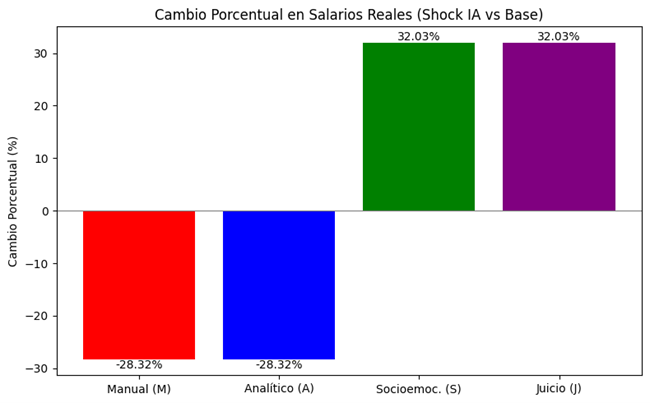
\includegraphics[width=0.7\linewidth]{views/entrega2/41.png}
                        \caption{Cambio en Salarios por Tipo de Trabajador/Tarea}
                        \label{fig:grafsal}
                    \end{figure}

                    Si bien, el cambio de los salarios depende del valor de $\lambda$ que se utilice, en la g\'afica anterior podemos ver la tendencia general de un choque de automatizaci\'on sobre los salarios. Al reemplazar tareas manuales y anal\'iticas, la oferta de estos trabajadores aumenta, mientras que la demanda disminuye lo que hace que los salarios caigan, frente al escenario base. Mientras que para trabajadores en tareas socioemocionales y en tareas de juicio, la automatizaci\'on hace que su escasez relativa aumente, e incluso se puede pensar en posible complementariedad entre el nuevo capital y estos trabajadores que incremente su productividad y por ende presiones sus salarios al alza.
        
      \item \textbf{Impacto sobre Agregados vs. \(\lambda\):}
        \begin{itemize}
          \item \textbf{Cambio en Output (\(\%\Delta y\) – Azul, Eje Izquierdo):} El impacto positivo del shock de automatizaci\'on sobre el output es significativamente mayor cuando \(\lambda\) es alta, aumentando de forma monótona desde aproximadamente +42\% (para \(\lambda=1.1\)) hasta casi +88\% (para \(\lambda=3.0\)).
          \item \textbf{Cambio en Participación del Capital (\(\Delta s_K\) – Rojo, Eje Derecho):} El cambio en la participación del capital (en puntos porcentuales) aumenta con \(\lambda\), pasando de aproximadamente +31 puntos porcentuales (para \(\lambda=1.1\)) a +43 puntos porcentuales (para \(\lambda=3.0\)). Esto se debe a que, con \(A_k=1.2\) y \(\Gamma_k=0.3\) fijo, se cumple que
            \[
            s_K = A_k^{(\lambda-1)}\cdot \Gamma_k,
            \]
            de donde \(\Delta s_K = s_K - 0\) crece con \(\lambda\).
        \end{itemize}
    \end{itemize}

  \item \textbf{Interpretación de los Cambios en Relación con \(\lambda\):}
    \begin{itemize}
      \item \textbf{Efectos sobre Salarios:}
        \begin{enumerate}[label=\alph*)]
          \item \textbf{Cuando \(\lambda\) es baja (tareas poco sustituibles, alta complementariedad):} La estructura productiva es más rígida. La pérdida de tareas para M y A impacta severamente sus salarios, ya que su trabajo es menos sustituible, mientras que las tareas no automatizadas (S y J) se vuelven cuellos de botella, generando grandes primas salariales.
          \item \textbf{Cuando \(\lambda\) es alta (tareas muy sustituibles):} La economía es más flexible. Aunque M y A pierden tareas, el impacto en sus salarios se amortigua gracias a: 
            \begin{enumerate}[label=\roman*)]
              \item Un aumento general en la productividad (\(y\)) que se transmite a todos los factores.
              \item Una menor criticidad de las tareas perdidas en la receta global de producción, lo que disminuye la prima por escasez en S y J.
            \end{enumerate}

            \begin{figure}[H] 
                \centering
                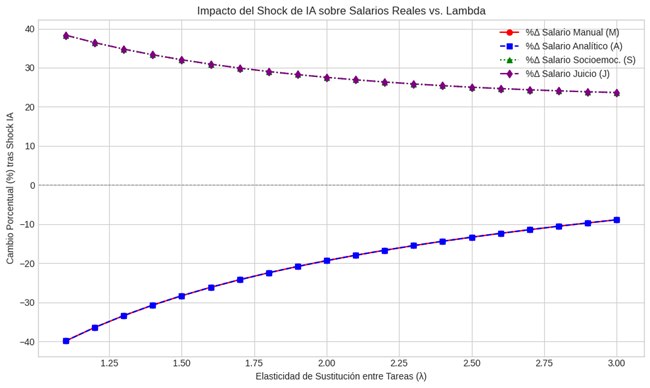
\includegraphics[width=0.7\linewidth]{views/entrega2/61.png}
                \caption{Impacto del Shock en Salarios  vs. Lambda}
                \label{fig:graflamb}
            \end{figure}
            Esta gr\'afica resume las relaciones planteadas anteriormente, como se puede observar entre m\'as pequeño sea lambda, la diferencia entre el aumento del salario para las tareas S y J y la caída del salario para las tareas M y A, es mayor. A medida que el valor de la elasticidad aumenta la brecha se va cerrando debido a que las tareas se vuelven m\'as sustituibles, lo que reduce la ca\'ida en el salario para los trabajadores M y A, y a su vez mitiga el aumento del salario para los trabajadores S y J. La linea azul en este caso representa el salario anal\'itico y manual,  mientras que la linea morada representa el salrio de tareas socioemocionales o de juicio.
        \end{enumerate}
        
      \item \textbf{Efectos sobre Agregados:}
        \begin{itemize}
          \item \textbf{Output (\(y\)):} Una \(\lambda\) alta facilita la reorganización de la economía para aprovechar al máximo el factor automatizado (sustituir trabajo por capital en tareas TR/TA), lo que incrementa las ganancias de productividad.
          \item \textbf{Participación del Capital (\(s_K\)):} Con \(A_k > 1\), una mayor \(\lambda\) amplifica el efecto del aumento de productividad del capital, haciendo que \(A_k^{(\lambda-1)}\) crezca más rápidamente y, junto a la cuota fija \(\Gamma_k\), incrementa la participación del capital en el ingreso total.
        \end{itemize}
            \begin{figure}[H] 
                \centering
                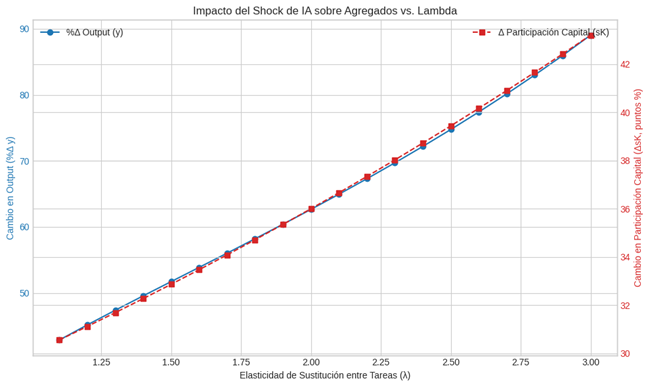
\includegraphics[width=0.7\linewidth]{views/entrega2/62.png}
                \caption{Impacto del Shock vs. Lambda}
                \label{fig:graflamb}
            \end{figure}
            En la gr\'afica podemos ver que mayores niveles de $\lambda$ llevan a incrementos mayores en la participaci\'on del capital, como en la producci\'on final. Como se explico anteriormente, esto se debe a que un mayor $\lambda$ incrementa la productividad general del capital $A_k$.
    \end{itemize}
    
  \item \textbf{Relación con la Evidencia Empírica:}
    \begin{itemize}
      \item \textbf{Estimaciones de \(\lambda\):}
        \begin{itemize}
          \item La literatura ha estimado que la elasticidad de sustitución puede variar según el nivel de agregación y la metodología, pudiendo ser baja (ej. \(< 1.5\text{--}2.0\)) o alta (más allá de \(2.0\text{--}2.5\)).
          \item Si la elasticidad es baja, el modelo predice efectos distributivos muy fuertes y ganancias agregadas modestas.
          \item Si la elasticidad es alta, se predicen mayores ganancias de productividad y efectos sobre la desigualdad salarial menos extremos.
          \item Es importante comparar el rango explorado (1.1 a 3.0) con estimaciones empíricas para evaluar la plausibilidad de los resultados.
        \end{itemize}

        
        
      \item \textbf{Tendencias Observadas:}
        \begin{itemize}
          \item \textbf{Polarización Salarial:} La evidencia en países desarrollados muestra que han aumentado los salarios en ocupaciones de alta habilidad y se han estancado o caído en ocupaciones de habilidad media, lo cual es consistente con la caída de M/A y el aumento de S/J.
          \item \textbf{Participación del Capital:} Se ha observado un aumento en la participación del capital en el ingreso nacional, en línea con el hecho de que \(\Delta s_K > 0\) y aumenta con \(\lambda\).
          \item \textbf{Crecimiento de la Productividad:} Aunque el impacto de la automatizaci\'on en la productividad es debatido, el modelo predice incrementos sustanciales en \(y\), especialmente con \(\lambda\) alta.
        \end{itemize}
    \end{itemize}
    
  \item \textbf{Conclusión:} La estática comparativa variando \(\lambda\) en el modelo simplificado revela que la elasticidad de sustitución entre tareas es un parámetro fundamental. Una mayor sustituibilidad (\(\lambda\) alta) amplifica las ganancias de productividad y la participación del capital, atenuando la polarización salarial, mientras que una menor sustituibilidad (\(\lambda\) baja) limita las ganancias agregadas y exacerba la desigualdad salarial. Estas predicciones se alinean cualitativamente con las tendencias empíricas, siendo clave contrastarlas con estimaciones empíricas de \(\lambda\).
\end{itemize}

        \end{tcolorbox}
    
    \item Calibre su modelo y compare las predicciones con datos de alguna econom\'ia del mundo:
    \begin{itemize}
        \item Explique qué parámetros serán fijados, cuáles se estimarán y de qué fuentes provienen los datos.
        \item Discuta brevemente cómo la calibración permite comparar las predicciones del modelo con datos reales.
    \end{itemize}

        \begin{tcolorbox}[title= Soluci\'on 6]

            La calibración es un proceso fundamental en la modelización económica que consiste en asignar valores numéricos a los parámetros de un modelo teórico para que sus predicciones, en un estado estacionario, coincidan o se aproximen lo máximo posible a datos observados en una economía real específica en un momento determinado. Este proceso ``ancla'' el modelo a la realidad, permitiendo luego realizar simulaciones que parten de una base empíricamente relevante.

            En este ejercicio, se calibró el modelo simplificado estable para replicar características de la economía estadounidense alrededor del año 2024. El proceso implicó los siguientes pasos:

\begin{enumerate}
    \item \textbf{Selección y Obtención de Targets Empíricos: } Variables clave del modelo cuyos valores en el equilibrio deben coincidir con los datos observados.
    \begin{itemize}
        \item Participaciones Laborales por Tipo ($l_g$): proporción del empleo total correspondiente a cada tipo de trabajador (M, A, S, J).
        \item Salarios Relativos ($w_g/w_A$): salarios promedio o medianos relativos al tipo A.
        \item Participación del Capital en el Ingreso ($s_K$): fracción del ingreso nacional que corresponde a la remuneraci\'on del capital.
    \end{itemize}

    \item \textbf{Fuentes de Datos y Procesamiento}
    \begin{itemize}
        \item \textbf{Datos de Tareas y Habilidades (O*NET)}:
        \begin{itemize}
            \item Se utilizaron bases de datos abilities.xlsx, skills.xlsx, work\_activities.xlsx, work\_context.xlsx. Estas bases contienen puntuaciones detalladas sobre la importancia o el nivel de diversas habilidades, capacidades, actividades y contextos laborales para cientos de ocupaciones estandarizadas (códigos SOC). 
            \item Se seleccionaron proxies específicos para M, A, S, J. Basados en la descripcion de cada `Element Id'
            \item Se calcularon índices normalizados (Z-scores). Para cada dimensi\'on y ocupaci\'on O*NET, promediando los valores de las proxies correspondientes
        \end{itemize}

        \item \textbf{Datos de Empleo y Salarios (OEWS)}:
        \begin{itemize}
            \item Se empleó la encuesta OEWS (national\_M2024\_dl.xlsx). Esta fuente proporciona datos sobre el empleo total (TOT\_EMP) y diversas medidas salariales (media, mediana, percentiles, anual y por hora) para cada ocupación detallada (código SOC) a nivel nacional.
            \item Se tomó la mediana salarial anual (A\_MEDIAN) como medida principal.
        \end{itemize}

        \item \textbf{Merge y Asignación de Tipo}:
        \begin{itemize}
            \item Fusión de datos O*NET y OEWS procesados.
            \item 713 ocupaciones comunes.
            \item Se asigno cada ocupaci\'on al tipo de trabajador correspondiente.
        \end{itemize}

        \item \textbf{Cálculo de Targets}:
        \begin{itemize}
            \item $l_g$ suma del empleo total de las ocupaciones asignadas a cada tipo g y dividiendo por el empleo total agregado en las 713 ocupaciones..
            \item $w_g/w_A$ basado en salario mediano ponderado por empleo para cada tipo g, dividido por el salario mediano ponderado del tipo A.
        \end{itemize}

        \item \textbf{Participación del Capital ($s_K$)}:
        \begin{itemize}
            \item Valor placeholder de 0.400, basado en fuentes externas (NIPA, PWT, literatura académica).
        \end{itemize}
    \end{itemize}

    \item \textbf{Parámetros Fijados:}
    \begin{itemize}
        \item $\lambda$: Elasticidad de sustitución entre tareas fijada en 1.5. Se toma de estudios econométricos previos o se fija en un valor plausible para el análisis.
        \item $A_A$: Productividad general del trabajo analítico, normalizada a 1.0.
        \item $A_k$: Productividad general del capital, fijada en 1.2. Este valor influye en la relación entre $s_K$ y $\Gamma_k$, y debe ser distinto de 1 para que $s_K$ varíe con lambda. Su valor exacto podría también ser objeto de calibración o análisis de sensibilidad.
        \item $L_g$: Ofertas laborales iguales a los targets $l_g$ observados. Esto asume que la oferta total de trabajo en la economía se normaliza a 1, y las $l_g$ representan las proporciones efectivas de cada tipo.
    \end{itemize}

    \item \textbf{Parámetros Estimados - Calibraciones}
    \begin{itemize}
        \item $\Gamma_k^{base}$ y $\Gamma_g^{base}$: Inferidos para ser consistentes con los targets.
        \item $A_M$, $A_S$, $A_J$: Calculados mediante fórmulas analíticas de salarios relativos. Valores obtenidos:
        \begin{itemize}
            \item $A_M \approx 0.1085$
            \item $A_S \approx 0.4253$
            \item $A_J \approx 2.0004$
        \end{itemize}
    \end{itemize}
\end{enumerate}

\textbf{Comparaci\'on de la predicci\'on con los datos:} \\
La calibración conecta el modelo teórico con los datos o tendencias observadas en el mundo real.

\begin{itemize}
    \item \textbf{Establecimiento de una Base Realista}:
    \begin{itemize}
        \item Al forzar el equilibrio base del modelo a coincidir con características clave observadas en la economía (como las participaciones laborales, la estructura salarial relativa y la participación del capital), la calibración asegura que cualquier simulación o análisis contrafactual parte de un punto inicial empíricamente relevante. Sin calibración, los parámetros ``arbitrarios'' podrían generar un estado base muy alejado de la realidad, haciendo que las predicciones de shocks o políticas sean poco creíbles.
    \end{itemize}

    \item \textbf{Evaluación Cualitativa y Cuantitativa}: El modelo calibrado puede usarse para simular fen\'omenos, o choques y ver como responden las variables.
    \begin{itemize}
        \item Comparación con tendencias observadas: dirección y magnitud relativa de cambios.
        \item Comparación con estudios econométricos: elasticidades y efectos cuantitativos.
    \end{itemize}

    \item \textbf{Entendimiento de Mecanismos}:
    \begin{itemize}
        \item Si las predicciones del modelo calibrado se alinean razonablemente bien con la realidad, esto da credibilidad a los mecanismos internos del modelo como explicaciones potenciales de los fenómenos reales. Si no se alinean, sugiere que faltan ingredientes importantes en el modelo o que la calibración necesita refinarse.
    \end{itemize}

    \item \textbf{Limitaciones}: Es importante recordar que la comparación siempre es imperfecta. La calibración misma depende de supuestos (elección de targets, parámetros fijos, estructura del modelo simplificado, regla de distribución de Gammas base). El modelo es una simplificación y no captura toda la complejidad del mundo real (heterogeneidad, fricciones, dinámica). Por lo tanto, la comparación suele ser más útil para evaluar consistencia cualitativa, órdenes de magnitud relativos y la plausibilidad de los mecanismos, que para buscar una replicación numérica exacta de los datos.
\end{itemize}

En suma, el proceso de calibración permitió asignar valores a las productividades relativas ($A_g$) en el modelo simplificado, asegurando que su estado base sea consistente con datos empíricos clave de EE.UU. 2023 ($l_g$, $w_g/w_A$, $s_K$). Esto proporciona una base fundamentada para simulaciones y para comparar cualitativamente las predicciones del modelo sobre fenómenos como la automatizaci\'on con la evidencia empírica disponible sobre crecimiento y distribución del ingreso.

        \end{tcolorbox}
    
    \item Utilice su modelo para realizar un análisis contrafactual:
    \begin{itemize}
        \item Proponga al menos un escenario alternativo (por ejemplo, un cambio en la política institucional, un shock tecnológico o variaciones en preferencias culturales) y analice sus implicaciones para el crecimiento económico.
        \item Discuta cómo su modelo ayuda a entender las consecuencias de estos cambios y qué limitaciones podría tener el enfoque.
    \end{itemize}

        \begin{tcolorbox}[title= Soluci\'on 7]
        Este punto utiliza el modelo económico calibrado para explorar las implicaciones de escenarios alternativos, distintos al estado base o al shock tecnológico inicialmente considerado. El objetivo es analizar cómo cambios hipotéticos (shocks tecnológicos de diferente intensidad o cambios institucionales/políticos simulados) afectan las predicciones del modelo, en particular respecto al crecimiento económico (cambios en el output agregado y), y discutir tanto la utilidad del modelo para entender estas consecuencias como sus limitaciones inherentes.
            \begin{enumerate}[label=(\alph*)]

\item \textbf{Marco del Análisis: Modelo Calibrado y Equilibrio Base} 

Se parte del modelo simplificado estable desarrollado previamente, cuyos parámetros fueron calibrados utilizando el \emph{Enfoque 2}, el cual asegura la consistencia con los \emph{targets} empíricos de participaciones laborales $(l_g)$, salarios relativos $(w_g/w_A)$ y, crucialmente, la participación del capital $(s_K)$ para la economía de referencia (EE.\,UU., $\sim$2024).

\begin{itemize}
  \item \textbf{Parámetros Calibrados}: Se utiliza el conjunto \texttt{calibrated\_params\_sk} que incluye $\lambda = 1.5$, $A_A = 1.0$, $A_k = 1.2$ y los valores calibrados $A_M \approx 0.1085$, $A_S \approx 0.4253$, $A_J \approx 2.0004$, junto con las ofertas laborales $L_g$ fijadas según las $l_g$ empíricas.
  \item \textbf{Gammas Base}: Se emplean las cuotas de tarea base inferidas (\texttt{Gammas\_base\_calib}) consistentes con $s_K = 0.4$:\; $\Gamma_k \approx 0.365$, $\Gamma_A \approx 0.115$, $\Gamma_S \approx 0.156$, $\Gamma_J \approx 0.033$, $\Gamma_M \approx 0.331$.
  \item \textbf{Equilibrio Base}: Al resolver el modelo con estos parámetros y gammas se obtiene:  
    \begin{itemize}
      \item Output: $y_base=0.5869$
      \item Participación del capital: $s_K=0.4000$
      \item Salarios: $w_M=0.2470$, $w_A=0.5178$, $w_S=0.3894$, $w_J=0.6524$
    \end{itemize}
\end{itemize}

\item \textbf{Escenarios Contrafactuales Propuestos}\\[2pt]
Se analizaron tres escenarios alternativos respecto al equilibrio base:

\begin{enumerate}
  \item \textbf{CF1 – Shock de automatizaci\'on leve}: se automatizan tareas TR hasta $0.05$ y TA hasta $0.30$.
  \item \textbf{CF2 – Shock de automatizaci\'on severo}: se automatizan TR hasta $0.20$ y TA hasta $0.45$.
  \item \textbf{CF3 – Mejora en habilidades socioemocionales}: se incrementa $A_S$ en 10\% (de $0.4253$ a $0.4678$) manteniendo las mismas gammas.
\end{enumerate}


\item \textbf{Implicaciones para el Crecimiento Económico y otros resultados}

\begin{itemize}
  \item \textbf{CF1 (Shock leve)}
    \begin{itemize}
      \item $\%\Delta y = -17.83$; fuerte contracción del output.
      \item $s_K = 0.1095$ (–29\, punto porcentuales).
      \item Salarios: $w_M$ –37.3\%, $w_A$ +26.7\%, $w_S$ +20.2 \%, $w_J$ +238.8\%.
      \item \emph{Interpretación}: resultado contraintuitivo. Sugiere que, dentro de la estructura específica de este modelo calibrado (con alto $Gamma_k$ base y productividades $A_g$ muy heterogéneas), una reasignación "pequeña" de tareas desde trabajadores de baja productividad calibrada (M, A) hacia capital (con $A_k=1.2$, pero que ya realiza muchas tareas) puede generar, contraintuitivamente, una pérdida neta de eficiencia agregada según la función CES. Este resultado debe tomarse con extrema cautela, pues podría ser un artefacto de la calibración o indicar una fragilidad del modelo simplificado ante pequeñas perturbaciones alrededor de una base con alta participación inicial del capital inferida.
    \end{itemize}

  \item \textbf{CF2 (Shock severo)}
    \begin{itemize}
      \item $\%\Delta y = +21.80$; crecimiento sustancial.
      \item $s_K = 0.4382$ (+3.82pp).
      \item Salarios: $w_M$ –67.6\%, $w_A$ –34.6\%, $w_S$ +56.2\%, $w_J$ +340.4\%.
      \item \emph{Interpretación}: Este escenario se alinea mejor con las expectativas cualitativas. Una automatizaci\'on m\'as fuerte impulsa la productividad agregada pero a costa de exacerbar enormemente la desigualdad salarial. La magnitud extrema del aumento de $w_J$ refleja la alta sensibilidad de este grupo (escaso en $L_J$ y $Gamma_J$, pero con $A_J$ calibrado muy alto) a cambios en el equilibrio general.
    \end{itemize}

  \item \textbf{CF3 (Mejora $A_S$ + 10 \%)}
    \begin{itemize}
      \item $\%\Delta y = +2.65$; crecimiento modesto, como resultado directo del aumento de productividad en el grupo S (que representa $\sim25\%$ del empleo).
      \item $s_K$ sin cambio $(0.4000)$, ya que la asignación de tareas y $A_k$ no cambiaron.
      \item Salarios: $w_S$+5.05\%, reflejando su mayor productividad; otros trabajadores +1.76\%, se benefician del crecimiento econ\'omico.
      \item \emph{Interpretación}: Este escenario ilustra cómo una política enfocada en mejorar las habilidades de un grupo específico puede generar beneficios agregados y tener efectos derrame positivos (aunque pequeños) sobre otros trabajadores en este marco.
    \end{itemize}
\end{itemize}

\item \textbf{Discusión: Utilidad del Modelo y Limitaciones}

\begin{itemize}
  \item \textbf{¿Cómo ayuda el modelo?} A pesar de las simplificaciones realizadas para lograr estabilidad, el modelo calibrado sirve como un "laboratorio cuantitativo" para explorar las implicaciones de diferentes escenarios bajo una estructura económica consistente. Permite:
    \begin{itemize}
      \item \emph{Cuantificar trade‑offs}: magnitudes para crecimiento, salarios y participación del capital.
      \item \emph{Comparar escenarios}: revela no linealidades (CF1 vs.\ CF2) y permite evaluar como la intensidad de un choque afecta los resultados.
      \item \emph{Evaluar políticas}: cambios en parámetros influenciables por pol\'iticas p\'ublicas y mirar su efecto en el mercado (ej.\ $A_S$).
      \item \emph{Predicciones condicionales}: ``Si ocurre X, esperaríamos Y'', útiles para la planificación y el debate informado, siempre reconociendo las bases del modelo..
    \end{itemize}
  \item \textbf{Limitaciones}
    \begin{itemize}
      \item \textbf{Reasignación de tareas exógena:} La principal limitación es que la reasignación de tareas en los shocks de automatizaci\'on (CF1, CF2) es impuesta externamente, no surge de una decisión económica endógena dentro de la simulación. El modelo calcula las consecuencias de la reasignación, no el proceso de adopción.
      \item \textbf{Supuestos de calibración no observables directamente:} La calibración base (Opción 2) replicó los targets, pero se basó en supuestos sobre la distribución de tareas (Gammas base inferidas) que no son directamente observables. Los resultados cuantitativos dependen de estos supuestos.
      \item \textbf{Parámetros clave fijos:} Valores clave como lambda y $A_k$ se mantuvieron fijos. Un análisis de sensibilidad a estos parámetros sería necesario para evaluar la robustez de los resultados.
      \item \textbf{Estática comparativa:} El análisis compara equilibrios antes y después del shock, sin modelar la trayectoria dinámica de ajuste, que podría implicar costos o efectos diferentes a corto/largo plazo.
      \item \textbf{Alta agregación:} El modelo es altamente agregado (un sector, cuatro tipos de trabajo homogéneos dentro de cada grupo), omitiendo heterogeneidad intra-grupo, fricciones del mercado laboral, geografía, etc., que son relevantes en la realidad.
    \end{itemize}
\end{itemize}

\end{enumerate}

\noindent\textbf{Conclusión}: El análisis contrafactual con el modelo simplificado y calibrado ofrece información cuantitativa sobre los efectos de shocks tecnológicos y políticas en el crecimiento y la distribución del ingreso. Aunque los resultados deben interpretarse con cautela, el modelo es una herramienta útil para explorar mecanismos económicos y formular predicciones condicionales sobre las dinamicas de automatizaci\'on y políticas relacionadas.

        
        \end{tcolorbox}
    
\end{enumerate}

\nocite{*}
\printbibliography

\section*{Disclaimer}
\textit{Este documento fue producido con la asistencia de herramientas de inteligencia artificial (ChatGPT y Claude AI) para escribir el código LaTeX y para mejorar aspectos de redacción y claridad en las respuestas. Posterior a la utilización de estas herramientas, hemos revisado y editado cuidadosamente todo el contenido y asumimos responsabilidad completa por el mismo.}

\end{document}



